\chapter{The Data}

After collecting the data, we must process it, decide whether or not to keep it, and if so use the data to reconstruct the collision event. The data is then placed on a computing grid, and can later be accessed for offline analysis. High-energy physics analyses also make use of vast amounts of simulated Monte Carlo events, which can be from either Standard Model or hypothetical processes.

\section{Object and Event Reconstruction}

The first step after data collection is to decide whether or not the event contains anything of interest. This is done via a trigger system~\cite{ATLAS_triggers}, shown in Figure~\ref{fig:triggers}.

\begin{figure}[htbp]
    \centering
    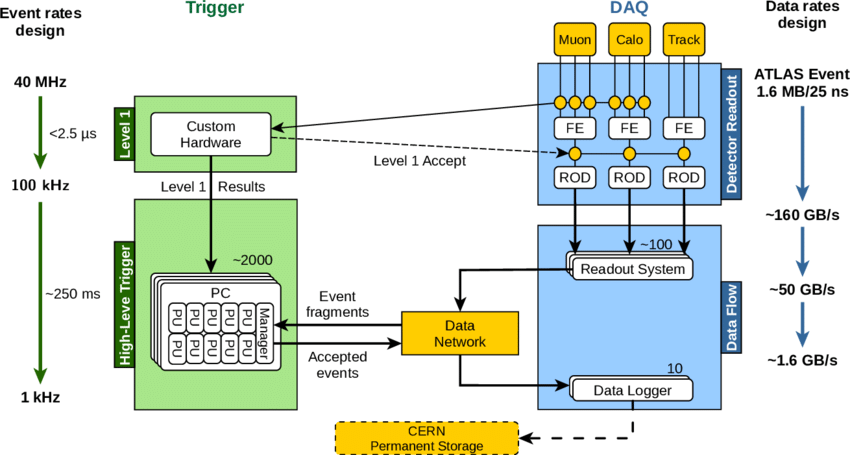
\includegraphics[width=\linewidth]{Images/ATLAS/triggers.png}
    \caption{The ATLAS trigger system. Figure from~\cite{ATLAS_triggers_figure}.}
    \label{fig:triggers}
\end{figure}

The data is first reduced from an average rate of 40 MHz to about 100 kHz via the Level-1 Triggers. These triggers are hardware-based, and take rough information from the calorimeters and muon spectrometers. They use simple algorithms to quickly check the data, using \pt\ thresholds to identify interesting events. These triggers also identify regions of interest (ROIs) for downstream use.

Next comes the High-Level Triggers (HLTs). These use offline algorithms along with the data passed in Level-1 ROIs to reconstruct objects, which have to pass various \pt\ requirements based on the trigger menu. Low-\pt\ object triggers are often prescaled, meaning that only a fraction of events passing those triggers are saved to disk. The rate is reduced to about 1 kHz after this point, making it possible to write events to disk.

In the Run-II upgrade of ATLAS, the event rate is raised high enough that we have to insert a new step in between the Level-1 and HLT triggers, using firmware on the inner detector to rapidly reconstruct tracks. I worked a bit on this proposed system, called the Fast TracKer (FTK), as will be discussed later in the thesis.

After this, we start running object reconstruction algorithms on the data~\cite{ATLAS_TDR}. We start by using information from the inner detector to reconstruct tracks. These tracks are then used to reconstruct vertices, and to determine a primary vertex, from which the highest-energy collision products are coming from. An event typically has one primary vertex (also called a hard-scatter vertex), and many pileup vertices, with much softer (less-energetic) interactions.

Primary objects like electrons and muons are reconstructed first, followed by jets, which are showers of particles. Various tools can also be applied to objects at this time to check for things like isolation (whether the object has other decay products around it) or b-tagging (whether a jet is the product of a bottom quark). After jet reconstruction we have overlap removal, where objects are compared against each other to make sure they weren't double-counted by multiple reconstruction algorithms. The final objects are also used to calculate \MET\ (missing energy), which is the energy vector in the transverse plane that would have to be added to the event to make it have a total energy of zero.

After the events are reconstructed, the data is stored on a worldwide computing network called the Grid~\cite{Grid}. Individual users can download data from the Grid onto their own workspaces, using it in their analyses.

\section{Data and Monte Carlo}

Actual collision events are commonly referred to as data, while simulated events are known as Monte Carlo (MC). This refers to the Monte Carlo sampling techniques commonly used to generate these artificial events. In high-energy analyses, we use MC events for many purposes. They allow us to develop and test our analysis techniques. They can let us look at individual processes, such as $Z\rightarrow\ell\ell$, which is useful for many purposes. They can also let us simulate hypothetical events, based on various Beyond-the-Standard-Model (BSM) models.

MC events in ATLAS are generated using the process in Figure~\ref{fig:MC_process}. Here we'll cover some of the major steps of the process. First an event is produced by a generator such as Herwig or Pythia, which calculates the physics processes in a collision, including hadronization and decays, initial and final state radiation, QCD processes, etc. The simulation step, which uses Geant4, uses the detector geometry to calculate what would happen to the produced particles as they propagate through the system. Digitization turns the event into a set of readout signals from the detector components. The resulting events are then fed into the normal reconstruction steps, which are the same for data and MC events.

\begin{figure}[htbp]
    \centering
    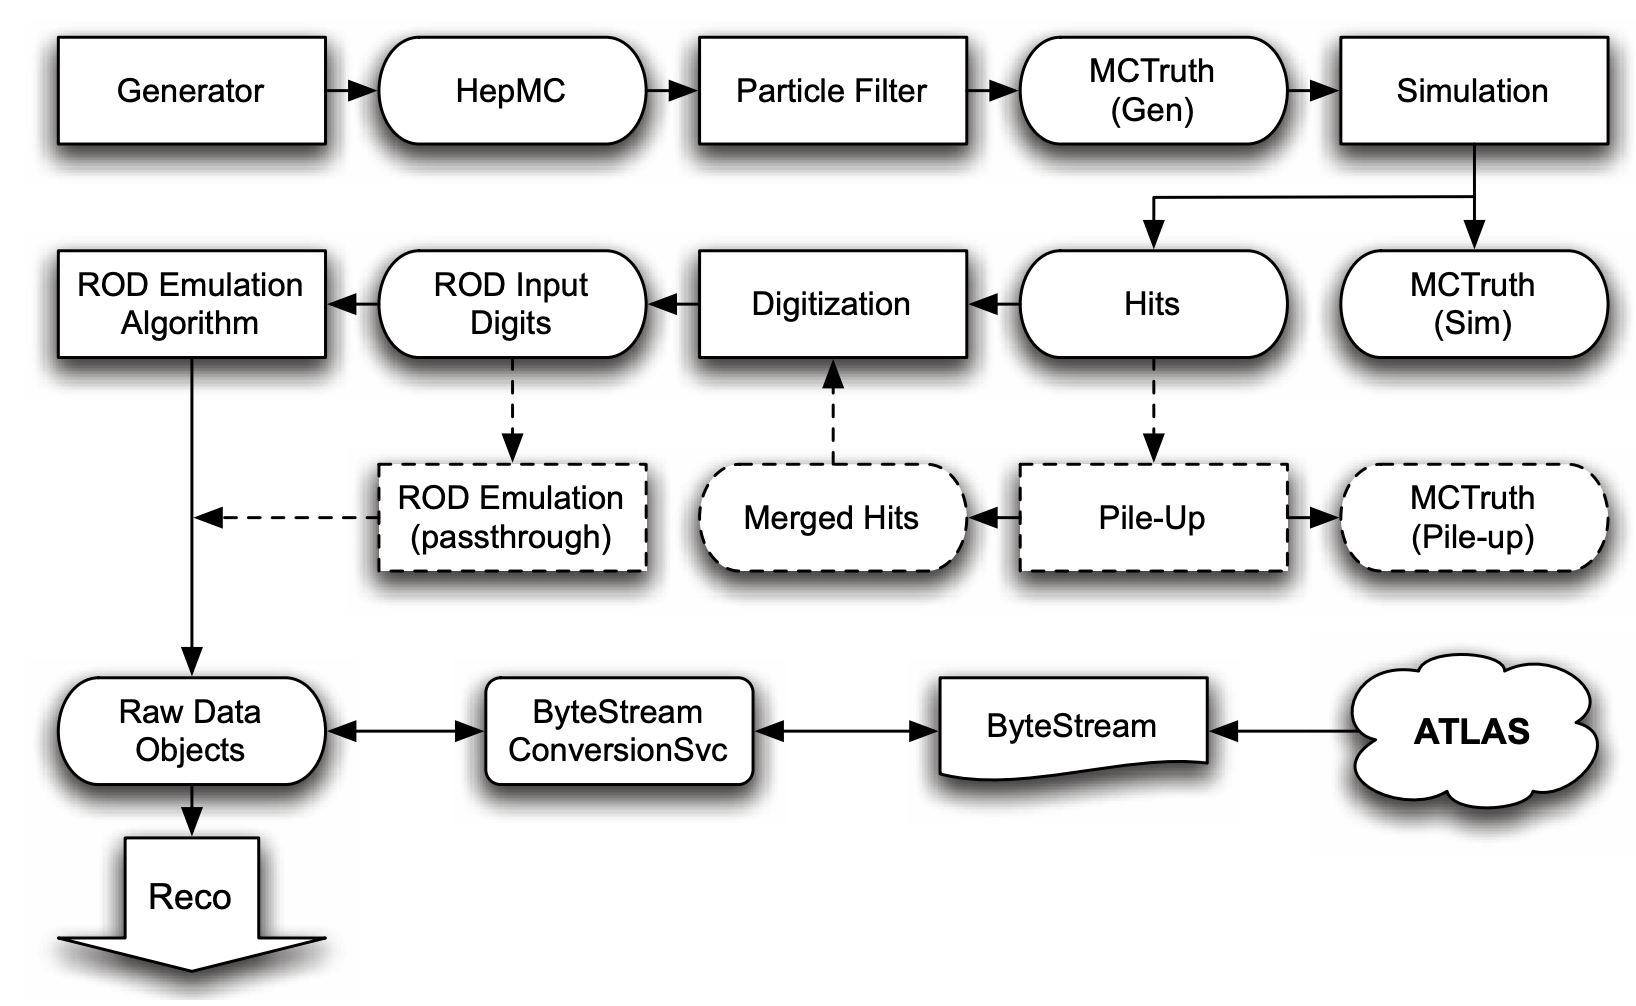
\includegraphics[width=\linewidth]{Images/ATLAS/MC.png}
    \caption{The ATLAS MC production pipeline. Figure from~\cite{ATLAS_computing_TDR}.}
    \label{fig:MC_process}
\end{figure}